\documentclass[12pt,letterpaper,titlepage]{report}
\usepackage{fontspec}
\defaultfontfeatures{Mapping=tex-text}
\usepackage{xunicode}
\usepackage{xltxtra}
\usepackage{enumitem}
\setmainfont{Times New Roman}
\usepackage{amsmath}
\usepackage{amsfonts}
\usepackage{amssymb}
\usepackage{multicol}
\usepackage{solarized-light}
\usepackage{paracol}
\usepackage{multirow}
\usepackage{graphicx}
\graphicspath{{img/}}
\usepackage{karnaugh-map}
\usepackage[margin=0.65in]{geometry}
\author{Jacob Abel}
\title{%
	Homework 9
	\\\large ECE2504 CRN:82729
}

%\renewcommand{\lstlistingname}{Combinational Circuit}
%\renewcommand{\lstlistlistingname}{List of \lstlistingname s}

\begin{document}
\maketitle
\begin{raggedright}
\raggedcolumns
\paragraph{Question 1:}
(4 pts) Recall the structural Verilog description of a ripple carry adder you wrote in class. Compile and simulate your description in Quartus. Apply combinations that check out the rightmost full adder for all eight input combinations; this also serves as a check for the other full adders. Submit the output waveform. Note that you will also need to assign inputs for the other three full adders – all 9 inputs and 5 outputs should be shown in your simulation. Choose your input values to include all eight possible combinations for the least significant full adder.
\begin{figure}[ht]
\centering
\includegraphics[width=\textwidth, height=\textheight, keepaspectratio=true]{hw9p1}
\caption{Ripple Carry Adder Simulation Waveform}
\end{figure}

\lstinputlisting[
	language=Verilog, 
	caption=4-bit Ripple Carry Adder
]{src/hw9p1.v}
\clearpage

\paragraph{Question 2:}
(4 pts) Draw the logic diagram that corresponds to the following structural Verilog description. 

\lstinputlisting[
	language=Verilog, 
	caption=Combinational Circuit 1
]{src/hw9p2.v}
\begin{figure}[ht]
\centering
\includegraphics[width=\textwidth, height=\textheight, keepaspectratio=true]{hw9p2}
\caption{Combinational Circuit 1 Logic Diagram}
\end{figure}

\clearpage

\paragraph{Question 3:}
(8 pts)
\begin{enumerate} [noitemsep, label=\alph*)]
\item Using the Verilog description in the previous problem as a framework, write a structural Verilog description of the circuit shown below. 
\item Compile and simulate the circuit in Quartus. Submit the waveform showing all inputs and outputs.
\end{enumerate}
\begin{figure}[ht]
\centering
\includegraphics[width=\textwidth, height=\textheight, keepaspectratio=true]{hw9p3a}
\caption{Problem 3 Logic Diagram}
\end{figure}
\clearpage

\lstinputlisting[
	language=Verilog, 
	caption=Problem 3 Structural Verilog Description
]{src/hw9p3.v}
\begin{figure}[ht]
\centering
\includegraphics[width=\textwidth, height=\textheight, keepaspectratio=true]{hw9p3b}
\caption{Problem 3 Simulation Waveform}
\end{figure}

\clearpage
\paragraph{Question 4:}
\begin{enumerate} [noitemsep, label=\alph*)]
\item (6 pts) Draw the logic diagram that represents minimum two‐level logic needed to implement the following Verilog dataflow description.
\item (1 pt) what type of circuit is this ? (i.e. what does it do?)
\end{enumerate}

\lstinputlisting[
	language=Verilog, 
	caption=Combinational Circuit 2 
]{src/hw9p4.v}
\begin{center}
\begin{karnaugh-map}[4][4][4][$cd$][$ab$][$ef$]
  \maxterms{0,3,5,6,8,11,13,16,19,22,24,27,35,37,38,43,45,51,54,59}
  \autoterms[1]
  \implicantedge{0}{0}{8}{8}[0,1]
  \implicantedge{3}{3}{11}{11}[0,1,2,3]
  \implicant{6}{6}[0,1,2,3]
  \implicant{5}{13}[0,2]
\end{karnaugh-map}
\end{center}
\vspace{-1cm}
\begin{align*}
(a'+b+c+e)(b+c'+d')(b'+c+d'+f)(a+b'+c'+d)
\end{align*}
\clearpage
\begin{figure}[ht]
\centering
\includegraphics[width=\textwidth, height=\textheight, keepaspectratio=true]{hw9p4}
\caption{Combinational Circuit 2 Logic Diagram}
\end{figure}

\clearpage

\paragraph{Question 5:}
(3 pt) Determine the (2‐input) gate count and propagation delay for circuit diagram you found for the previous problem. Use a form similar to HW8, Problem 1 (where $t_{pdNOT}$ = propagation delay of an inverter, $t_{pdAND}$ = propagation delay of a 2‐input AND gate, and $t_{pdOR}$ = propagation delay of a 2‐input OR gate).

\paragraph{Question 6:}
(3 pt) Determine the (2‐input) gate count and propagation delay for circuit diagram described in Figure 3‐33 (below). Use a form similar to HW8, Problem 1 (where $t_{pdNOT}$ = propagation delay of an inverter, $t_{pdAND}$ = propagation delay of a 2‐input AND gate, and $t_{pdOR}$ = propagation delay of a 2‐input OR gate).

\lstinputlisting[
	language=Verilog, 
	caption=4-to-1-Line Multiplexer 
]{src/hw9p6.v}

\clearpage
\paragraph{Question 7:}
(8 pts) Using the conditional dataflow concept from Figure 3‐33 (above), complete the following Verilog dataflow description for an 3x8 decoder using the conditional operator. Compile and simulate your description with a set of inputs that are a good test for the selection function it performs. Submit the waveform.
\lstinputlisting[
	language=Verilog, 
	caption=3x8 Decoder 
]{src/hw9p7.v}
\begin{figure}[ht]
\centering
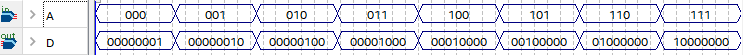
\includegraphics[width=\textwidth, height=\textheight, keepaspectratio=true]{hw9p7}
\caption{3x8 Decoder Simulation Waveform}
\end{figure}

\clearpage
\paragraph{Question 8:}
(8 pts) Using the module definitions from Problem 1 (4‐bit ripple carry adder) and Problem 6 (Figure 3‐33), implement the arithmetic circuit shown in the Case Study 2 Sample Solution. You will need to instantiate the ripple carry adder module and as many muxes as you need into your Verilog model. Compile and simulate the circuit in Quartus. Submit the waveform showing all inputs and outputs. Use the following inputs.
\begin{center}
\begin{tabular}{|c|c|c|c|}
\hline 
$R_1R_0$ & $c_0$ & $X$ & $Y$ \\ \hline 
00 & 0 & \multirow{7}{*}{0100} & \multirow{7}{*}{1101} \\  
00 & 1 &  &  \\  
01 & 0 &  &  \\  
01 & 1 &  &  \\  
10 & 0 &  &  \\  
10 & 1 &  &  \\  
11 & 0 &  &  \\ \hline 
\end{tabular} 

\end{center}

\begin{figure}[ht]
\centering
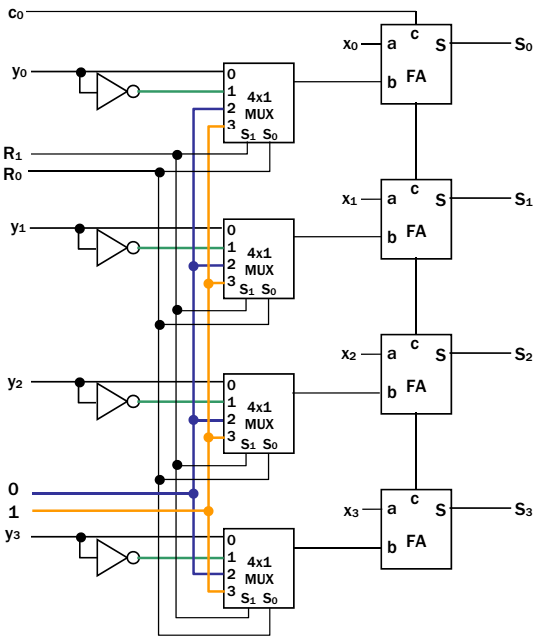
\includegraphics[width=0.5\textwidth, height=\textheight, keepaspectratio=true]{hw9p8a}
\caption{Case Study 2 Logic Diagram}
\end{figure}
\clearpage
\lstinputlisting[
	language=Verilog, 
	caption=Case Study 2
]{src/hw9p8.v}
\begin{figure}[ht]
\centering
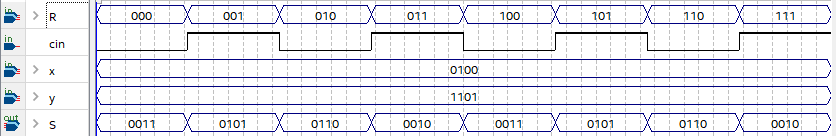
\includegraphics[width=\textwidth, height=\textheight, keepaspectratio=true]{hw9p8b}
\caption{Case Study 2 Simulation Waveform}
\end{figure}
\clearpage

\paragraph{Question 9:}
(8 pts) Determine the (2‐input) gate count and propagation delay for
\begin{enumerate} [noitemsep, label=\alph*)]
\item the circuit you designed in the previous problem.
\item the circuit shown below. 
\end{enumerate}
Use a form similar to HW8, Problem 1 (where $t_{pdNOT}$ = propagation delay of an inverter, $t_{pdAND}$ = propagation delay of a 2‐input AND gate, and $t_{pdOR}$ = propagation delay of a 2‐input OR gate).
\lstinputlisting[
	language=Verilog, 
	caption=Combinational Circuit 3
]{src/hw9p9.v}

\vspace{\fill}
\noindent
GRADING SCALE
\medskip

Total: 53 pts
\bigskip

\def\arraystretch{1.5} 
\begin{tabular}{ | l | c | c | c | c | c | c | c | c | } \hline
Pts          & 0  & 6  & 13 & 19 & 26 & 32 & 39 & 46     \\\hline
Letter Grade & D- & D  & C- & C  & B- & B  & A- & A      \\\hline
\end{tabular}
\end{raggedright}
\end{document}